\startchapter{Background Material}
\label{chapter:background}

\newlength{\savedunitlength}
\setlength{\unitlength}{2em}
This chapter provides a short summary of the material which is relevant to the subject of this research. Starting with the concepts underlying 
implicit and deformable tissue modeling and an outline of continuum mechanics and finite element concepts, the chapter will conclude by reviewing closely related 
deformable models presented in the litrature. 

\section{Implicit Modeling}
Implicit surfaces are two-dimensional, geometric shapes that exist in three-dimentional space; they can be defined based on discrete data, 
radial basis functions, offset surfaces, algebraic surfaces, level sets or distance fields to skeletal geometric primitives \cite{Bloomenthal1997}.
Independently of its origin, an implicit surface can be defined as a level-set function $F:\mathbb{R}^3 \rightarrow \mathbb{R}$ where the surface 
and the volume can be defined as following:

\begin{equation}
S = \left\{M = (x,y,z) \in \mathbb{R}^3 | F(x,y,x) = c\right\}
\end{equation}

\begin{equation}
V = \left\{M = (x,y,z) \in \mathbb{R}^3 | F(x,y,x) \geq c\right\}
\end{equation}

$c$ is a constant and is called the \textit{iso-value} which is set to $0.5$ in our system. For each point in space if the field is greater than
$c$ the point is considered inside the model otherwise outside. 

Most of the primitives used in the \blob are built from geometric skeletons, which are incorporated in many implicit modeling software packages 
such as BlobTree.net \cite{de2008blobtree} or ShapeShop \cite{Schmidt2006}. They are ideally suited to prototype shapes of arbitrary topology 
\cite{Bloomenthal1997}. In general these works conclude that the use of skeletal primitives can lead to a simple and intuitive user modelling 
methodology. The basic building block of a skeletal primitive is a skeleton $S$. To create a skeletal primitive the distance-field $dS$ of the 
volume encapsulating the shape has to be computed as described in \cite{Barbier2004}. The distance field is a volume of scalar values which is 
not bounded as the distance itself can be infinitely large.

By modifying $dS$ with a field function $g$, it can be bound to a finite range. Usually the function maps the distances to the range $[0, 1]$, 
where the field has values of 1 at the skeletons and 0 after a certain distance to the skeleton (usually at distance 1). A discussion of field 
function appears in \cite{shirley2009graphics}. Skeletal implicit primitives are combined using binary operators, which are applied pair wise to 
field-values f, and represented by a node in the BlobTree, whose children are either primitives or operators themselves.
Field values are computed for the child-nodes and combined to yield a new value according to the operator type. This makes it possible to go beyond 
the classical Boolean operators, and define general blend operators that e.g. create smooth transitions between shapes. The most common operator 
that creates a smooth transition between several values is called the summation blend \cite{Bloomenthal1997}:

\begin{equation}
F_A(x, y, z)=\sum_{i=1}^{i=N_A}F_i(x, y, z)
\end{equation}

Where an implicit model $A$ is generated by summing the influences of $N_A$ skeletal elements: 
The field value due to an skeletal element at a point in 3D space is computed as filtered distance to its skeleton 
where the filter function (i.e. falloff function) is defined as follows \cite{Wyvill1999}: 

\begin{equation}
g_\mathrm{wyvill}(x)= \left\{ \begin{array}{rl}
 1 &\mbox{ if $x\leq0$} \\
 (1-x^2)^3 &\mbox{ if $0<x<1$}\\
  0 &\mbox{ if $x\geq1$}  
  \end{array} \right.
\label{eq:WyvillFunc}
\end{equation}

In equation \ref{eq:WyvillFunc}, $x$ is clamped to the range $[0,1]$. This polynomial smoothly decreases from 1 to 0 over the valid range, with zero
tangents at each end. An important property of this skeletal primitive definition is that the scalar field is \textit{bounded}, meaning that $f=0$
outside some sphere with finite radius. Bounded fields guarantee local influence, preventing changes made to a small part of a complex model from
affecting distant portions of the surface. Local influence preserves a \textquotedblleft principle of least surprise\textquotedblright that is critical for interactive modeling.  
Normals can be derived from gradients which are computed by evaluating 4 field values and performing a numerical approximation:

\begin{equation}
\nabla F(x,y,z)=\left\{ \begin{array}{rl}
 F(x+\delta,y,z)-f \\
 F(x, y +\delta,z)-f \\
 F(x, y, z+\delta)-f \\
  \end{array} \right. 
\label{eq:Normal}
\end{equation}

Where $f = F(x,y,z)$ is the field at point $(x,y,z)$.
% $fv = F(x,y,z)$ be the field at a point:
%$\nabla F(x,y,z)=\frac{1}{\delta}\left( F(x+\delta,y,z)-fv \right)$

Each skeletal primitive has a bounded region of influence in space. For each node in the tree an
axis-aligned bounding box is computed which is used to trivially reject those field queries that 
are outside the box. The bounding box of the entire model is computed as the union of all primitive
nodes bounding boxes.

For evaluating the field  at a point $P$ in a \blob model such as the one shown in figure (\ref{fig:CoffeeMugBlobTree}), 
the tree structure should be traversed from root to leaves recursively. 
Each operator combines the values of its children according to its type.
For example, for a simple blend the values are summed. A leaf node represents
a primitive,  and returns the value by applying equation~\ref{eq:WyvillFunc} to 
  the distance of $P$ from the primitive.

\begin{figure}[htb]
  \centering
  % the following command controls the width of the embedded PS file
  % (relative to the width of the current column)
  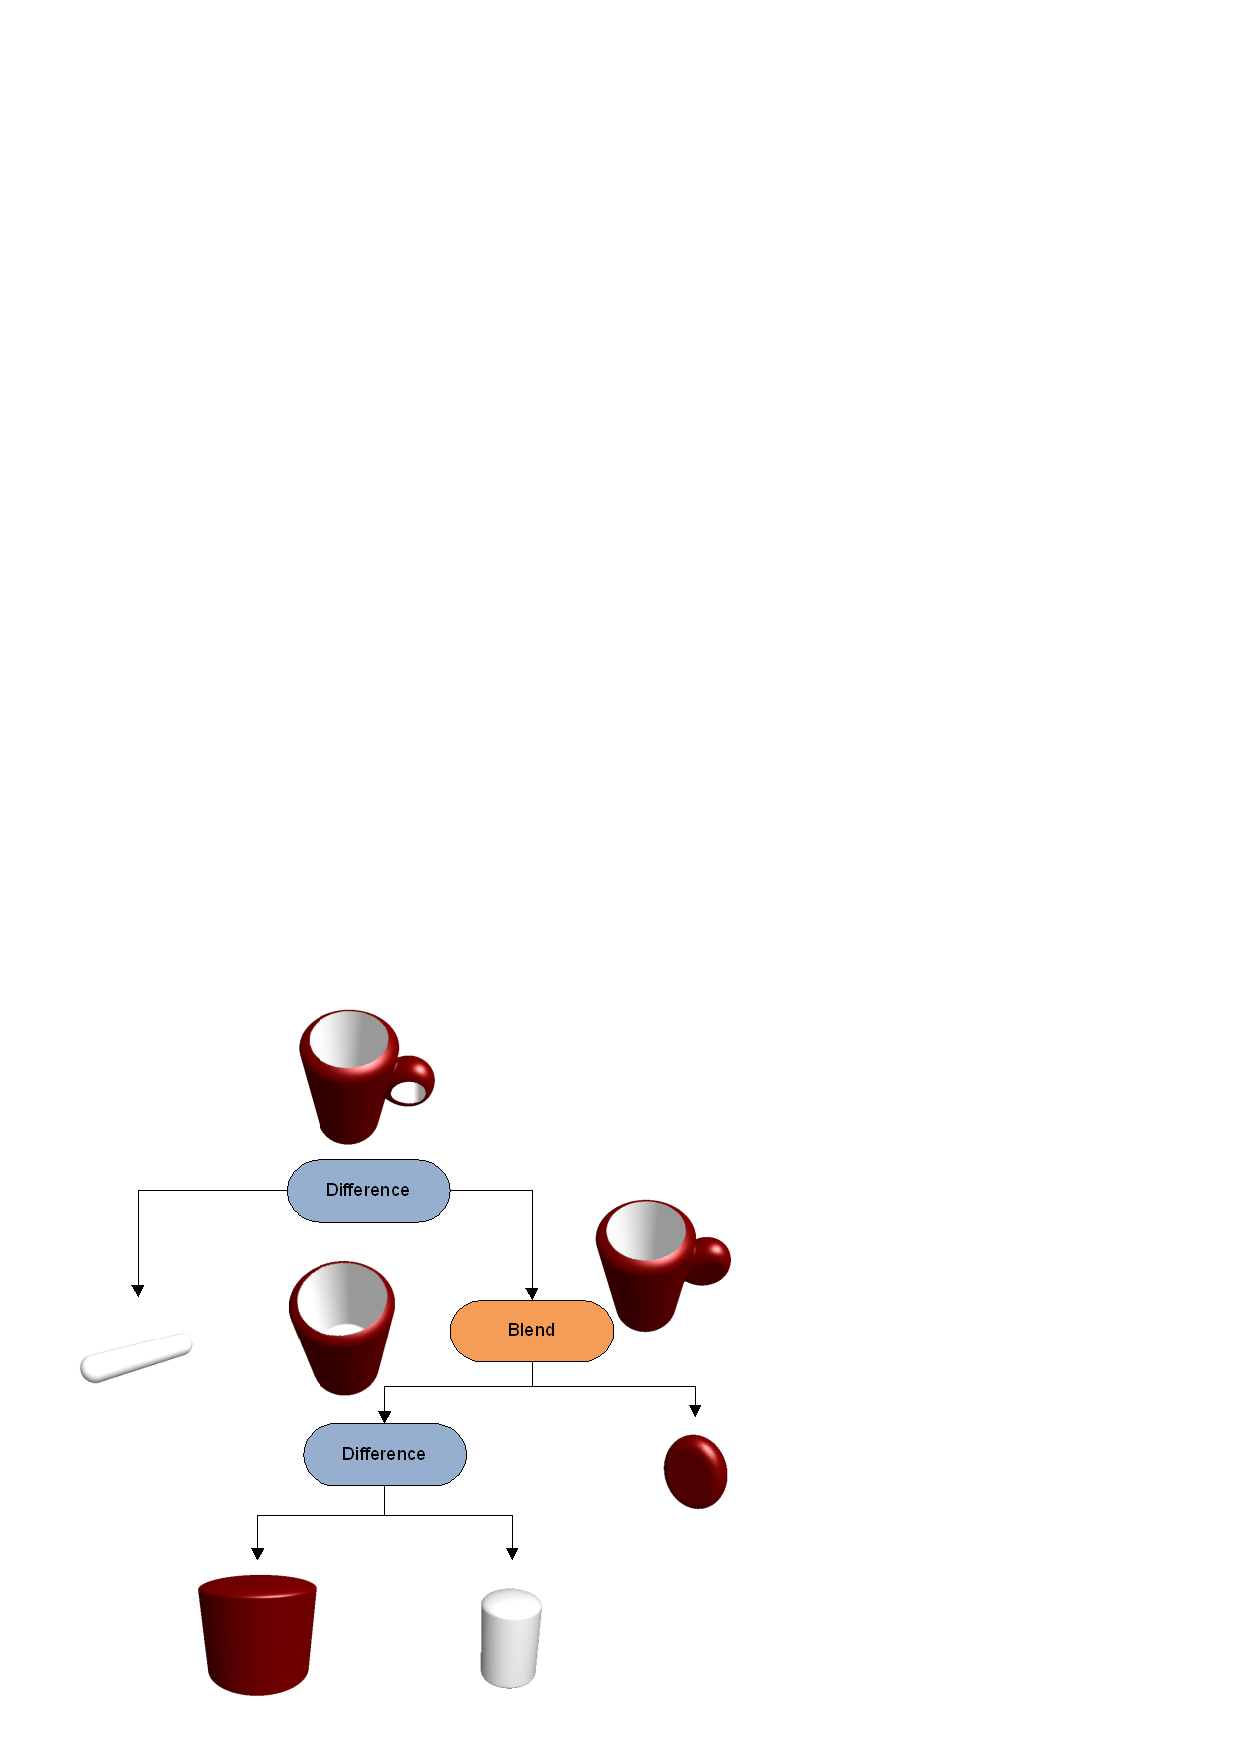
\includegraphics[width=1.0\linewidth]{figures/CoffeeMugBlobTree}
  \caption{\label{fig:CoffeeMugBlobTree}
           \blob structure of a coffee mug created with CSG and skeletal implicit primitives.}
\end{figure}

%As the tree gets deeper and the number of primitives increase the computation 
For visualization purposes the \blob is queried numerous times to evaluate the field. As suggested in \cite{SWG2005} 
accelerating field computation will have a large impact on the overall surface extraction process. 

\section{Sweep Surfaces and Sketching}
Implicit primitives in our system are created from skeletons which are simple geometrical shapes such as points, line segments or 
polygons from which volumetric distance fields are created. In order to support more complex geometries \textit{Schmidt} \etal proposed the
implicit sweep objects technique where the 2D shape sketched by the user is sampled and an implicit approximation is created from 
the sample points \cite{Schmidtc}. This is done by fitting a thin-plate spline as a base shape to the sampled points using variational 
interpolation \cite{Turk1999}. One advantage of creating the base shape using variational interpolation is that the resulting implicit 
field is $C^2$ continuous, a property needed when the shape is involved in several blending operations \cite{barthe2004controllable}.

A continuous 2D scalar field is created from several field value samples $(\mathbf{m}_i, v_i)$, where $\mathbf{m}_i$ describes the 
position of the sample and $v_i$ is the desired field. The thin-plate spline used to create the variational 
implicit field $f_c(\mathbf{u})$ is defined in terms of these points weighted by corresponding coefficients $w_i$ combined with a polynomial 
$P(u) = c_1u_x +c_2u_y +c_3$.

\begin{equation}
f_c(\mathbf{u}) = \sum_{i \in N} w_i(\|\mathbf{u}-\mathbf{m}_i\|)^2ln(\|\mathbf{u}-\mathbf{m}_i\|)+P(\mathbf{u}) 
\label{eq:thinplatespline}
\end{equation}

The weights $w_i$ and coefficients $c_1$, $c_2$, and $c_3$ are found by solving a linear system defined by evaluating 
equation \ref{eq:thinplatespline} at each known solution $f_c(\mathbf{m}_i)=v_i$.
The resulting thin plate spline can then be used as the basis of several different primitives:

\begin{itemize}
 \item Inflated Objects
 \item Swept object along a trajectory
 \item Revolving object around axis
\end{itemize}

These sketched objects can then be used in the same way as the standard skeletal implicit primitives to create unique 3D shapes. Such 
unique shapes were not possible to create in previous collaborative environments, especially given this technique’s small memory footprint 
needed to transfer the information.

\section{Continuum Mechanics Concepts}
Continuum biomechanics for soft tissue simulation deals with the movement of soft materials when subjected to applied forces. 
The motion of a continuous and deformable solid can be described by a continuous displacement field resulting from a set of 
forces acting on the solid body. A displacement \textit{field} implies a continuous variation of displacement with position. 
The continuous displacement field can be time-independent or time-dependent. The initial unloaded state of material is referred to 
as the \textit{reference} or \textit{undeformed} state as the displacements are zero everywhere. The material then reconfigures due to 
applied loads and reaches an equilibrium state referred to as \textit{deformed} state. The concepts of \textit{strain}, a measure of length
change or displacement gradient, and \textit{stress}, the force per unit area on an infinitesimally small plane surface within the material, 
are of fundamental importance for continuum biomechanics of soft tissues. 

The formulation of models in continuum mechanics consists of three parts:

\begin{enumerate}
 \item Kinematics: Geometric description of the deformation
 \item Dynamics: A formulation of the equations of motion
 \item Constituitive formulation: Description of the material properties
\end{enumerate}





\setlength{\unitlength}{\savedunitlength}
